\setcounter{chapter}{0}

%----------------------------------
\chapter{Introduction}\hyperdef{part}{intro}{}\label{ch:intro}
%----------------------------------


\section{Model Description}
%%% Incorporate the intro paragraph that used to begin this Chapter here.
%%% This is location of the true introduction where you explain why this
%%% model exists.
%%% Identify the Model context within JEOD.

The orbital elements class provides a representation of the translational
orbital state of an orbital body in standard Keplerian orbital elements.  In
addition, this class provides methods for converting between the Keplerian
orbital elements and planet centered inertial Cartesian position and velocity
vectors.  The methods in this class are primarily based on the methods
presented in Vallado \cite{Vallado} although some modifications have been made
to increase the numerical accuracy of the routines in limiting cases.

In the object design sense, the \OrbitalElement\ is almost completely independent from the remainder of JEOD.  The \OrbitalElement\ is
used to initialize DynBodyInitOrbit, to construct OrbElemDerivedState and to perform initializations in the verification sims of the DerivedState class.

This documentation describes the design of the \OrbitalElement\
in detail.  The orbital element class borrows heavily from published work
on the design of algorithms for converting between Keplerian orbital elements
and Cartesian position and velocity vectors.

This documentation covers a complete guide for the use of the orbital element
class.  It presents the mathematical equations and algorithms used to create
the orbital element class source code, defines requirements on the code,
reports the results of test cases run the verify and validate the model, and
contains a guide for the use of the orbital element class in a Trick
simulation environment.

\section{Document History}
%%% Status of this and only this document.  Any date should be relevant to when
%%% this document was last updated and mention the reason (release, bug fix, etc.)
%%% Mention previous history aka JEOD 1.4-5 heritage in this section.
%%% Mention that JEOD.pdf is the parent document.

\begin{tabular}{||l|l|l|l|} \hline
\DocumentChangeHistory
\end{tabular}

\section{Document Organization}
This document is formatted in accordance with the
NASA Software Engineering Requirements Standard~\cite{NASA:SWE}
and is organized into the following chapters:

\begin{description}
%% longer chapter descriptions, more information.

\item[Chapter 1: Introduction] -
This introduction contains three sections: description of model, document history, and organization.
The first section provides the introduction to the \OrbitalElementDesc\ and its reason
for existence.  It also contains a brief description of the interconnections with other models, and
references to any supporting documents.  The second section displays the history of this document which includes
author, date, and reason for each revision. The final
section contains a description of how the document is organized.

\item[Chapter 2: Product Requirements] -
Describes requirements for the \OrbitalElementDesc.

\item[Chapter 3: Product Specification] -
Describes the underlying theory, architecture, and design of the \OrbitalElementDesc\ in detail.  It is organized in
three sections: Conceptual Design, Mathematical Formulations, and Detailed Design.

\item[Chapter 4: User Guide] -
Describes how to use the \OrbitalElementDesc\ in a Trick simulation.

\item[Chapter 5: Verification and Validation] -
Contains \OrbitalElementDesc\ verification and validation procedures and results.

\end{description}

%----------------------------------
\chapter{Product Requirements}\hyperdef{part}{reqt}{}\label{ch:reqt}
%----------------------------------
This model shall meet the JEOD project requirements specified in the
\hyperref{file:\JEODHOME/docs/JEOD.pdf}{part1}{reqt}{JEOD} top-level document.

%%% Format for the model Requirements is open.  It should include requirements for this model
%%% only and use requirment tags like the one below.
%\requirement{...}
%\label{reqt:...}
%\begin{description}
%  \item[...]\ \newline
%    The documentation for the model shall include
%
%    \subrequirement{}
%    \label{reqt:...}
%      Software requirements specification.
%
%    ...
%
%  \item[title]\ \newline
%    text
%
%  ...
%
%\end{description}

%----------------------------------
\requirement{Cartesian to Element Conversion}
\label{reqt:cart_convert}
\begin{description}
  \item[Requirement:]\ \newline
     The \OrbitalElement\ shall be capable of taking in an arbitrary
     set of Cartesian position and velocity vectors and outputting the
     correct set of Keplerian orbital elements.
  \item[Rationale:]\ \newline
    This is one of the main two functions of the \OrbitalElement.

  \item[Verification:]\ \newline
    Test
\end{description}

\requirement{Element to Cartesian Conversion}
\label{reqt:elem_convert}
\begin{description}
  \item[Requirement:]\ \newline
     The \OrbitalElement\ shall be capable of taking in an arbitrary
     set of Keplerian orbital elements  and outputting the correct set
     of Cartesian position and velocity vectors.
  \item[Rationale:]\ \newline
    This is one of the main two functions of the \OrbitalElement.

  \item[Verification:]\ \newline
    Test
\end{description}

\chapter{Product Specification}\hyperdef{part}{spec}{}\label{ch:spec}
%----------------------------------

\section{Conceptual Design}
\subsection{Purpose and Scope}
The \OrbitalElement\ is a class whose methods convert between Keplerian orbital
elements and Cartesian position/velocity representations of the translational state.
This module is not a stand-alone program; rather, it is designed to be
incorporated into the Trick Simulation Environment, and applies to space
vehicles or objects whose states need to be converted between Cartesian
vectors and Keplerian orbital elements.

\subsection{Goals and Objectives}
The goal of the \OrbitalElement\ is to be able to convert between
any arbitrary set of orbital elements and Cartesian position and velocity
vectors with a high degree of accuracy and reliability.  That is the primary
function of this class.  A secondary function is for the \OrbitalElement\
to output error messages if for some reason it is unable to fulfill its
primary goal.


\section{Mathematical Formulations}
Conversion between Keplerian orbital elements and Cartesian position and
velocity is a well understood problem that has been solved many times.  There
are several methods that can be used with no clear distinction between them
in terms of computational loading and algorithm reliability.  A classic
technique used in many engineering applications is described in~\cite{Vallado}.
The algorithms presented in~\cite{Vallado} were initially implemented in Trick and
now constitute the \OrbitalElement.  A quick description of these
algorithms is presented here but for a more complete treatment, please see
\cite{Vallado}.

A satellite's translational state can be completely defined by using either
position and velocity information or classical Keplerian orbital elements.
It is advantageous to be able to use Keplerian elements for some applications
and position and velocity vectors for other applications.  Therefore, it is
important that the mission designer be able to convert between the two types
of state description quickly.  The simpler of the two conversions involves
determining the spacecraft position and velocity from a set of classical
orbital elements.

\subsection{Nomenclature}
The mathematical formulations in this chapter follow a common orbital element
nomenclature:

\begin{tabular}{@{\hspace{0.25in}} p{0.75in} p{5in}}
$p$      & The object's semi-parameter \\
$\nu$    & The object's true anomaly \\
$\mu$    & The gravitational body's gravitational constant \\
$\Omega$ & Right Ascension of the Ascending Node \\
$\omega$ & The argument of periapsis \\
$i$      & The orbital inclination of the body \\
$\lambda_{true}$ & The true longitude of the body \\
$\tilde{\omega}_{true}$ & The true argument of periapsis \\
$\vec{e}$              & The eccentricity vector \\
$\vec{r}$              & The Cartesian position vector \\
$\vec{v}$              & The Cartesian velocity vector \\
$\vec{h}$              & The angular momentum vector \\
$\vec{n}$              & The vector for the line of nodes \\
$I, J, K$               & The x, y, and z unit vector directions \\
\end{tabular}

\subsection{Position and Velocity to Orbital Elements}
If a user has access to a full set of Keplerian orbital elements, the
conversion from orbital element description to position and velocity
description is a simple process.  First, the position and velocity in the
perifocal coordinate system are determined and then they are rotated into
the inertial reference frame of interest (frequently J2000).

The position and velocity of the system in perifocal coordinates are functions
of the orbit's semi-parameter $p$, the orbital eccentricity $e$, the true anomaly
of the orbit $\nu$, and the gravitational parameter of the gravitational body $\mu$.  These parameters are used because a formulation for each is
defined regardless of the type of orbit (circular, eccentric, inclined,
parabolic, etc.).  The position values of the spacecraft in the perifocal
coordinate system can be calculated as shown in Equation \ref{peri_pos}.
\begin{equation}
\vec{r}_{PQW}=\begin{bmatrix} \frac{p\cos (\nu)}{1+e\cos (\nu)} \\
                              \frac{p\sin (\nu)}{1+e\cos (\nu)} \\
                              0 \end{bmatrix}
\label{peri_pos}
\end{equation}
The velocity of the spacecraft in the perifocal coordinate system is
then given by Equation \ref{peri_vel}.
\begin{equation}
\vec{v}_{PQW}=\begin{bmatrix} \sqrt{\frac{\mu}{p}}\sin (\nu) \\
                              \sqrt{\frac{\mu}{p}}(e+\cos (\nu) \\
                              0 \end{bmatrix}
\label{peri_vel}
\end{equation}
In the above equations, the parameter $e$ is the orbital eccentricity and is
defined as the magnitude of the eccentricity vector which is given in section
2.4.1 of~\cite{Vallado}.  The parameter $\nu$ is the true anomaly of the
spacecraft which is defined as the angle between the line from the primary
focus of the orbit to periapsis and the line from primary focus to spacecraft.
  This parameter is not always defined but a formulation can be used for these
special cases.  The parameter $p$ is the semi-parameter of the orbit and is
defined as the width of the orbit at the primary focus.  The parameter $\mu$
is the gravitational parameter of the primary body and is the gravitational
constant multiplied by the body's mass.

With the perifocal position and velocity vectors defined, the spacecraft
need only be rotated into the inertial system of interest.  This is
accomplished through use of a rotation matrix that is a function of the orbital
inclination $i$, the right ascension of the ascending node (RAAN) $\Omega$, and
the argument of periapsis $\omega$.  The values for the elements of this
rotation matrix are given in Equation \ref{p_j_rot}
\begin{equation}
\begin{bmatrix} \frac{IJK}{PQW} \end{bmatrix} =
   \begin{bmatrix} \cos(\Omega) \cos(\omega)-\sin(\Omega)\sin(\omega)\cos(i)
                 & -\cos(\Omega)\sin(\omega)-\sin(\Omega)\cos(\omega)\cos(i)
                 & \sin(\Omega)\sin(i) \\
                   \sin(\Omega)\cos(\omega)+\cos(\Omega)\sin(\omega)\cos(i)
                 & -\sin(\Omega)\sin(\omega)+\cos(\Omega)\cos(\omega)\cos(i)
                 & \cos(\Omega)\sin(i) \\
                   \sin(\omega)\sin(i)
                 & \cos(\omega)\sin(i)
                 & \cos(i)
   \end{bmatrix}
\label{p_j_rot}
\end{equation}
Now for certain cases, these parameters are not always defined.  For example,
with circular orbits, the argument of periapsis and true anomaly are not
defined because there is no periapsis point to provide reference.  There are a
set of rules that deal with these special cases and they are listed here.
\begin{itemize}
\item If orbit is circular and equatorial
   \begin{itemize}
   \item $\omega$ = 0.0
   \item $\Omega$ = 0.0
   \item $\nu$=$\lambda_{true}$
   \end{itemize}
\item If orbit is circular and inclined
   \begin{itemize}
   \item $\omega$ = 0.0
   \item $\nu$=$u$
   \end{itemize}
\item If orbit is elliptical and equatorial
   \begin{itemize}
   \item $\Omega$ = 0.0
   \item $\omega$ = $\tilde{\omega}_{true}$
   \end{itemize}
\end{itemize}
In the equations given above, some new parameters are introduced.  The
parameter $\lambda_{true}$ is the true longitude and is defined as the angle
between the coordinate frame x-axis and the spacecraft measured eastward from
the axis (towards y).  The parameter $u$ is the argument of latitude and is
angle between the ascending node and the spacecraft's position.  And lastly,
the parameter $\tilde{\omega}_{true}$ is the true longitude of periapsis and
is defined as the angle between the eccentricity vector and the x-axis.

With these equations and definitions, it is now possible to compute the
spacecraft state for any orbit.  These equations describe the algorithms used
in the \OrbitalElement\ and can be found in section 2.6 of~\cite{Vallado}.

\subsection{Orbital Elements from Position and Velocity}
The orbital elements of the spacecraft can be calculated using the
gravitational parameter of the primary body and the Cartesian position and
velocity vectors.  The algorithms for this conversion are relatively simple
and also very robust.  Similarly to how the equations from~\cite{Vallado} were
used for the position and velocity computation, there are algorithms in the
text for conversion from position and velocity to orbital elements.  These
algorithms are used in the code and are described briefly here.  For a more
complete treatment, please see~\cite{Vallado}.

First, several classic parameters must be calculated.  The spacecraft's angular
momentum is $\vec{h}$ and is defined as the cross product of the spacecraft's
position and velocity.  The parameter $h$ is the magnitude of this vector.
The spacecraft's line of nodes is denoted as $\vec{n}$ and it is the cross
product of the z-axis and the spacecraft's angular momentum.  The specific
energy of the system is $\xi$ and is defined as the potential energy of the
spacecraft subtracted from the kinetic energy.  The eccentricity vector is a
complex relation between position and velocity described by Equation
\ref{e_vec}.
\begin{equation}
\vec{e}=\frac{(v^2-\frac{\mu}{r})\vec{r}-(\vec{r}\cdot \vec{v})\vec{v}}{\mu}
\label{e_vec}
\end{equation}
The eccentricity $e$ is then just the magnitude of the vector value given in
Equation \ref{e_vec}.  Using these relations, four of the orbital elements
discussed above can be computed from the relations shown in Equation
\ref{orb_el}.
\begin{equation}
\begin{split}
&\cos(i) = \frac{h_K}{|\vec{h}|}\\
&\cos(\Omega) = \frac{n_I}{|\vec{n}|}
    \quad IF(n_j < 0) THEN \Omega = 360^o-\Omega\\
&\cos(\omega) = \frac{\vec{n}\cdot\vec{e}}{|\vec{n}||\vec{e}|}
    \quad IF(e_K<0) THEN \omega = 360^o-\omega\\
&\cos(\nu) = \frac{\vec{e}\cdot\vec{r}}{|\vec{e}||\vec{r}|}
    \quad IF(\vec{r}\cdot\vec{v}<0) THEN \nu = 360^o-\nu
\end{split}
\label{orb_el}
\end{equation}
In the above equations,
the subscripts indicate the direction of the vector.  For example, the value
$n_K$ is the z-component of the $\vec{n}$ vector.

The semi-major axis and semi-parameter have two different calculation methods
for use when the orbit is parabolic and when it is not.  These calculations
are show in Equation \ref{a_p_cal}.
\begin{equation}
\begin{split}
& IF\thickspace e \neq 1.0\thickspace THEN\\
&\qquad a=\frac{-\mu}{2\xi}\\
&\qquad p=a(1-e^2)\\
&ELSE\\
&\qquad p =\frac{h^2}{2}\\
&\qquad a= \infty
\end{split}
\label{a_p_cal}
\end{equation}
Once again, there are special cases for when the orbit is circular or equatorial.
These special rules are given in Equation \ref{spec_rul}.
\begin{equation}
\begin{split}
&Elliptical Equatorial \\
&\qquad \cos(\tilde{\omega}_{true})=\frac{e_I}{|\vec{e}|}
   \quad IF(e_J<0)THEN \thickspace \tilde{\omega}_{true} = 360^o-\tilde{\omega}_{true}\\
&Circular Inclined \\
&\qquad \cos(u)=\frac{\vec{n}\cdot\vec{r}}{|\vec{n}||\vec{r}|}
   \quad IF(r_K<0)THEN \thickspace u = 360^o-u\\
&Circular Equatorial\\
&\qquad \cos(\lambda_{true}) = \frac{r_I}{|\vec{r}|}
   \quad IF(r_J<0)THEN\lambda_{true}=360^o-\lambda_{true}
\end{split}
\label{spec_rul}
\end{equation}
These parameters function as a substitute for the argument of periapsis or the
true anomaly depending on the case.

With these equations, it is now possible to convert over from the Cartesian
position and velocity to the Keplerian orbital elements.  Once again, this is
a very brief description of the complete algorithms which can be found in
section 2.5 of~\cite{Vallado}.

\subsection{Solving Kepler's Problem}
Frequently, a mission designer needs to calculate the complete set of orbital
elements from a few of the available orbital elements.  This often entails
finding the solution to Kepler's equation.  The equations used in the code
convert between mean anomaly and the anomaly for the orbit.  The mean anomaly is
used such that if the orbit was circular, that is the anomaly it would have.
The orbital anomaly is then the angle formed between the line from the focus to the
periapsis and the position vector in the orbit.  So, for a circular orbit, the
orbital anomaly is always equal to the mean anomaly.  There is a version of Kepler's
equation for each orbit type (elliptical, parabolic, and hyperbolic).

So with these three equations, it is possible to determine all of the orbital
elements from a smaller set.  These equations represent a minor part of the
overall software model so they have not been included in this document.
However, if an algorithm check is desired, the algorithms from which the
\OrbitalElement\ have been copied can be located in section 2.2 of
\cite{Vallado}


\section{Detailed Design}
The \OrbitalElementDesc\ uses a single class to accomplish its purpose.  This
section describes the \OrbitalElement.
\subsection{Class Description}
The {\em orbital\_elements.h} file contains the class
used by the \OrbitalElementDesc\ source code.
A detailed description of the \OrbitalElement\ follows.

\subsubsection{Fields}
The public data fields of the \OrbitalElement\ are as follows:
\begin{itemize}
   \item Orbit Definition Parameters
\begin{itemize}
\item semi\_major\_axis: M     Semi-major-axis ($a$)
\item semiparam: M     Semiparameter ($p$)
\item e\_mag: --   Magnitude of eccentricity ($e$)
\item inclination: r     Orbit inclination ($i$)
\item arg\_periapsis: r     Argument of periapsis ($\omega$)
\item long\_asc\_node: r     Longitude of ascending node ($\Omega$)
\end{itemize}
   \item Orbital Position Parameters
\begin{itemize}
\item r\_mag: M     Magnitude of orbital radius
\item vel\_mag: M/s   Magnitude of orbital velocity
\item true\_anom: r     True Anomaly ($\nu$)
\item mean\_anom: r     Mean Anomaly ($M$)
\item mean\_motion: r/s   Mean motion of orbit ($n$)
\item orbital\_anom: r     Eccentric ($E$), Hyperbolic ($H$), or
                                       Parabolic ($B$) anomaly
\end{itemize}
   \item Working Parameters
\begin{itemize}
\item sin\_v: --    Sine of the true anomaly
\item cos\_v: --    Cosine of the true anomaly
\item orb\_energy: M$^2$/s$^2$ Specific orbital energy
\item orb\_ang\_momentum: M$^2$/s  Specific orbital angular momentum
\end{itemize}
\end{itemize}

\subsubsection{Methods}
In addition to the default constructor and the destructor,
the OrbitalElements class also contains the following member functions.

\paragraph{set\_object\_name}

This member function sets the name of the orbiting object.

\begin{itemize}
\item{return:} void - no return
\item{IN:}    const char * name - Orbital object name
\end{itemize}

\paragraph{get\_object\_name}

This member function returns the name of the orbital object.
\begin{itemize}
\item{return:} const char* The name of the orbital object
\item{IN:}    void -- no inputs
\end{itemize}

\paragraph{set\_planet\_name}

This member function sets the name of the planet.

\begin{itemize}
\item{return:} void - no return
\item{IN:}    const char * name - Planet name
\end{itemize}

\paragraph{get\_planet\_name}

This member function returns the name of the planet.
\begin{itemize}
\item{return:} const char* The name of the planet
\item{IN:}    void -- no inputs
\end{itemize}

\paragraph{from\_cartesian}

This function initializes fields of the \OrbitalElement\ which correspond
to Keplerian orbital elements based
on a position and velocity in planet-centered inertial coordinates
and the gravitational parameter of the primary

\begin{itemize}
\item{return:} int -- always returns $0$
\item{IN:}    double $\mu$ the gravitational parameter of the planet (product
of planetary mass and universal gravitational constant)
\item{IN:}    const double pos[$3$] The position of the orbital object
in planet-centered inertial coordinates
\item{IN:}   const double  vel[$3$] The velocity of the orbital object
in planet-centered inersial coordinates
\end{itemize}

\paragraph{to\_cartesian}

\begin{itemize}
\item{RETURN:}   int -- always returns $0$
\item{IN:}   $\mu$ The gravitational parameter of the planet
\item{OUT:}   double pos[$3$] The position of the orbital object corresponding
to the Keplerian orbital elements of this OrbitalElements object
\item{OUT:}   double vel[$3$]  The velocity of the orbital object corresponding to the Keplerian orbital
elements of this OrbitalElementsObject
\end{itemize}

\paragraph{nu\_to\_anomalies}

    This method calculates and sets the Mean Anomaly and the Eccentric, Hyperbolic, or
     Parabolic Anomalies, given the True Anomaly and eccentricity of
this OrbitalElements object

\begin{itemize}
\item{RETURN:}   int -- always returns $0$
\item{PARAMETERS:}   none
\end{itemize}

   \paragraph{mean\_anom\_to\_nu}

This method calculates and sets the true anomaly from the mean anomaly
and eccentricity of this OrbitalElements object.

\begin{itemize}
\item{RETURN:}   int -- always returns $0$
\item{PARAMETERS:}   none
\end{itemize}
\section{Inventory}

All \OrbitalElementDesc\ files are located in the directory
\$JEOD\_HOME/models/utils/orbital\_elements.
Tables~\ref{tab:source_files} to~\ref{tab:verification_files}
list the configuration-managed files in this directory.
\input{inventory}


%----------------------------------
\chapter{User Guide}\hyperdef{part}{user}{}\label{ch:user}
%----------------------------------
% The Analysis section of the user guide is intended primarily for users of pre-existing simulations.
% It contains:
% \begin{itemize}
% \item a description of how to modify \OrbitalElementDesc\ variables after the simulation
% has compiled, including an in-depth discussion of the input file,
% \item an overview of how to interpret (but not edit) the S\_define file,
% \item a sample of some of the typical variables that may be logged.
% \end{itemize}
%
% The Integration section of the user guide is intended for simulation developers.
% It describes the necessary configuration of the \OrbitalElementDesc\ within an
% S\_define file, and the creation of standard run directories.  The latter
% component assumes a thorough understanding of the preceding Analysis section of the user guide.
% Where applicable, the user may be directed to selected portions of Product Specification (Chapter \ref{ch:spec}).
%
% The Extension section of the user guide is intended primarily for developers
% needing to extend the capability of the \OrbitalElementDesc\.  Such users should have a
% thorough understanding of how the model is used in the preceding
% Integration section, and of the model
% specification (described in Chapter \ref{ch:spec}).
%
% \section{Analysis}
Although it is possible to run the \OrbitalElement\ from a Trick S\_define file, this is not a common usage in most
simulations.  Rather, the \OrbitalElement\ is typically employed as a conversion utility as in the definition of the
OrbElemDerivedState class.  The verification cases for the \OrbitalElement\
are run from an S\_define file using the test class OrbElemVer to store and log data as well as to exercise the to\_cartesian, from\_cartesian and mean\_anom\_to\_nu conversion methods of the \OrbitalElement.

The following are lines from an S\_define file which declare and initialize an \OrbitalElement.

\begin{verbatim}
   /* The only necessary structure for this test is ORBITAL ELEMENTS */
   utils/orbital: OrbitalElements orb_elem
      (orb_elem_ver/data/orb_elem_init.d);
\end{verbatim}

The test class OrbElemVer contains a single method which exercises the methods of the \OrbitalElement.  It's data consist of public fields for inertial position, velocity, gravitational parameter and a flag to determine which conversion is to be performed.
\begin{verbatim}
   Flag   to_cartesian; // --    Flag to determine which direction.
   double mu;           // M3/s2 Gravity constant for routine.
   double position[3];  // M     Pos vector for elem conversion.
   double velocity[3];  // M/s   Vel vector for elem conversion.
\end{verbatim}

The to\_cartesian variable determines if the conversion is going to
Cartesian from Keplerian elements or Keplerian elements to Cartesian.
If the to\_cartesian variable is set to True, the
OrbitalElements::to\_cartesian method is used:
\begin{verbatim}
   int OrbitalElements::to_cartesian( // RETURN: --  Return always zero.
      double mu,       // IN:  M3/s2  Gravitational parameter of planet.
      double pos[3],   // OUT: M      Orbital position vector of vehicle.
      double vel[3] ); // OUT: M/s    Orbital velocity vector of vehicle.
\end{verbatim}

If the to\_cartesian variable is set to False, the
OrbitalElements::from\_cartesian method is used:
\begin{verbatim}
   int OrbitalElements::from_cartesian( // RETURN: --  Return always zero.
            double mu,       // IN: M3/s2   Gravitational parameter of planet.
      const double pos[3],   // IN: M       Position vector of vehicle.
      const double vel[3] ); // IN: M/s     Velocity vector of vehicle.
\end{verbatim}

% \section{Integration}


% \section{Extension}


%----------------------------------
\chapter{Verification and Validation}\hyperdef{part}{ivv}{}\label{ch:ivv}
%----------------------------------

\section{Inspection and Verification}\label{sec:inspect}

\inspection{Data conversion}\label{inspect:data_conversion}
The \OrbitalElement\ contains the fields and methods needed to completely satisfy
\ref{reqt:elem_convert} and \ref{reqt:cart_convert}.

\section{Validation}\label{sec:test}

In this set of validation tests, 56 test cases were run in order to determine
that the system was performing nominally.  For each test bullet below, several
of those test cases are included as part of the testing description.  The code
and data files associated with these testing bullets can be found in the verif
directory inside of the orbital/dynamics directory.  Inside of the verif
directory, there is the SIM\_orb\_elem/SET\_test sub-directory which
contains all of the various testing directories.  They are all labeled with
the convention:

RUN\_T\#\_OE\_VER

In this convention, the \# ranges from 01-57 (There is one unused testing
directory).  The run numbers associated with a particular test are called out
in the test bullet.

\test{Circular Equatorial Orbits}\label{test:circ_equa_per}
\begin{description}
\item[Purpose:] \ \newline
The purpose of this test is to examine the performance of the orbital element
class when dealing with circular equatorial orbits.
\item[Requirements:] \ \newline
By passing this test, the \OrbitalElement\ partially satisfies
requirement~\ref{reqt:elem_convert} and partially satisfies
requirement~\ref{reqt:cart_convert}.
\item[Procedure:]\ \newline
This test is designed to test the conversion from Cartesian position and
velocity to orbital elements.  It tests the model's capabilities with respect
to circular, equatorial orbits.  These orbits are used to verify that the
code can correctly convert circular equatorial values and because the
determination of the correct results by hand is a trivial matter.
\item[Results:]\ \newline
Figure \ref{cir_eq_tab} shows the results computed for four different circular
orbits.  They all had the same radius of 7,378,145 m and velocity magnitude of
7,350.1 m/s.  The only difference was the direction of the position and velocity
vectors.

\begin{figure}[h]
\begin{center}
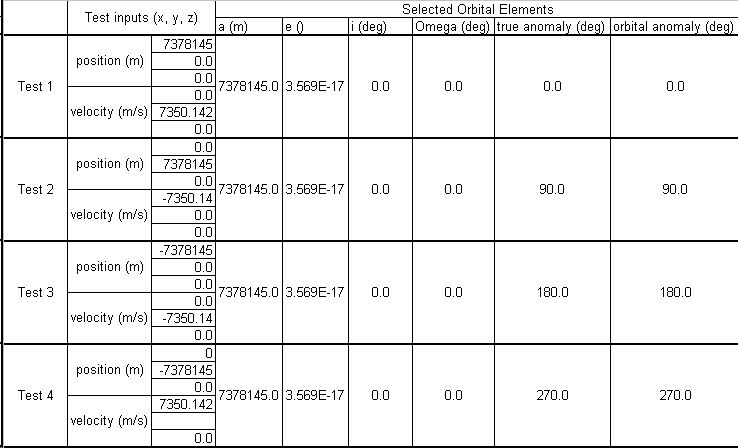
\includegraphics[height=85mm]{JPGfiles/circ_equa.jpg}
\caption{Table of Testing Results for Circular Equatorial Orbits}
\label{cir_eq_tab}
\end{center}
\end{figure}
This table shows nominal results for all sub-tests.  The presence of non-zero
values for the true anomaly would normally indicate problems because for
circular orbits, the true anomaly is undefined.  However, in the model, the
true anomaly variable is set to the value for the true longitude so that the
element to Cartesian computation can be used interchangeably.

One parameter not recorded in the above table but useful for the orbital
element class is the spacecraft mean motion.  This parameter is the
average angular velocity magnitude of the spacecraft over one orbit.
Because the angular velocity magnitude of the spacecraft remains constant
for the duration of the orbit, the instantaneous angular velocity is the
same as the mean motion.  The formula for the instantaneous angular velocity
of the spacecraft is given by Equation
\ref{sc_omega}.
\begin{equation}
\omega_sc = \frac{\vec{r} \thickspace x \thickspace \vec{v}}{|\vec{r}|^2}
\label{sc_omega}
\end{equation}
According to this equation as well as the position and velocity
magnitudes, the expected mean motion should be 9.9620E-4 rad/s.  The value
computed by the equations of motion matches this value to 13 digits of
precision.

Run directories:

01-04
\end{description}

\test{Circular Polar Orbits}\label{test:circ_pol_per}
\begin{description}
\item[Purpose:] \ \newline
The purpose of this test is to examine the performance of the orbital element
class when dealing with circular polar orbits.
\item[Requirements:] \ \newline
By passing this test, the \OrbitalElement\ partially satisfies
requirement~\ref{reqt:elem_convert} and partially satisfies
requirement~\ref{reqt:cart_convert}.
\item[Procedure:]\ \newline
This test is designed to test the conversion from Cartesian position and
velocity to orbital elements.  It tests the model's capabilities with respect
to circular, polar orbits.  These orbits are used to verify that the
code can correctly convert circular polar values and because the
determination of the correct results by hand is a trivial matter.
\item[Results:]\ \newline
Figure \ref{cir_eq_90} shows the results computed for four different circular
polar orbits.  They all had the same radius of 7,378,145 m and velocity
magnitude of approximately 7,350.1 m/s.  The only difference was the
direction of the position and velocity vectors.
\begin{figure}[h]
\begin{center}
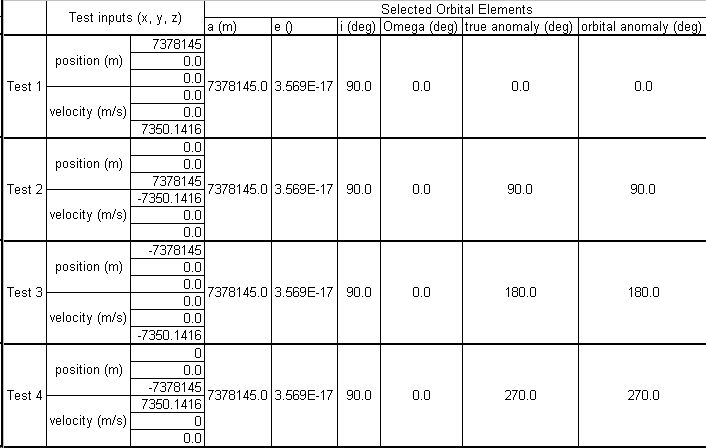
\includegraphics[height=85mm]{JPGfiles/circ_in_90.jpg}
\caption{Table of Testing Results for Circular Polar Orbits}
\label{cir_eq_90}
\end{center}
\end{figure}

Figure \ref{cir_eq_90} shows nominal results for all four of the sub-tests run.
Once again, there appears to be incorrect results when it outputs non-zero
values for the true anomaly but this is once again the case of another variable
being stored in the true anomaly portion of the structure.  In this case, the
stored parameter is argument of latitude $u$.  All of the other parameters are
the expected values.  Because the same radius and velocity magnitude was used,
the same mean motion of 9.962E-4 rad/s was observed with the same accuracy.

Run directories:

05-08
\end{description}

\test{Circular Inclined Orbits}\label{test:circ_inc_per}
\begin{description}
\item[Purpose:] \ \newline
The purpose of this test is to examine the performance of the orbital element
class when dealing with circular inclined orbits.
\item[Requirements:] \ \newline
By passing this test, the \OrbitalElement\ partially satisfies
requirement~\ref{reqt:elem_convert} and partially satisfies
requirement~\ref{reqt:cart_convert}.
\item[Procedure:]\ \newline
This test is designed to test the conversion from Cartesian position and
velocity to orbital elements.  It tests the model's capabilities with respect
to circular, inclined orbits.  These orbits are used to verify that the
code can correctly convert circular inclined values and because the
determination of the correct results by hand is a trivial matter.
\item[Results:]\ \newline
Figure \ref{cir_eq_45} shows the results computed for four different circular
inclined orbits.  They all had the same radius of 7,378,145 m and velocity
magnitude of approximately 7,350.1 m/s.  The only difference was the direction
of the position and velocity vectors.  This test case is slightly more complex
than the previous two test cases.  The basic orbit was a 30 degree inclined
orbit with the RAAN equal to zero degrees.  However, in order to test the
RAAN computation, all of the position and velocity vectors were rotated by
45 degrees to place the RAAN at 45 degrees.
\begin{figure}[h]
\begin{center}
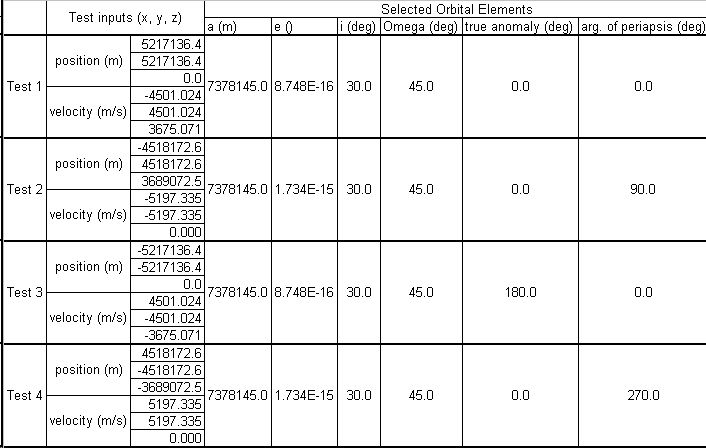
\includegraphics[height=85mm]{JPGfiles/cir_in_45.jpg}
\caption{Table of Testing Results for Circular Inclined Orbits}
\label{cir_eq_45}
\end{center}
\end{figure}
Figure \ref{cir_eq_45} shows nominal results for all four of the sub-tests run.
While this may not be clear for tests two and four, they do represent nominal
behavior despite the fact that the argument of periapsis value was non-zero.
With these tests, due to numerical precision of the computer, the eccentricity
was set higher than the eccentricity tolerance (1E-15) set in the source code.
Therefore, these orbits were treated as eccentric orbits and the argument of
periapsis was calculated.  This is not a problem.  The mean motion for this
test was also 9.962E-4 rad/s.

Run directories:

09-12

\end{description}

\test{Elliptical Orbits}\label{test:circ_ell_per}
\begin{description}
\item[Purpose:] \ \newline
The purpose of this test is to examine the performance of the orbital element
class when dealing with elliptical orbits of all types.
\item[Requirements:] \ \newline
By passing this test, the \OrbitalElement\ partially satisfies
requirement~\ref{reqt:elem_convert} and partially satisfies
requirement~\ref{reqt:cart_convert}.
\item[Procedure:]\ \newline
This test is designed to test the conversion from Cartesian position and
velocity to orbital elements.  It tests the model's capabilities with respect
to elliptical orbits of all inclinations.  The calculation of analytical
results for these orbits is more complicated than for other cases but it
is still possible.

In order to preserve the ability to validate the algorithms being tested,
equations from section 1.6 of~\cite{BMW} were used to compute the initial
conditions that would result in the desired orbital elements.  For this test,
there were constant eccentricity (.2) and constant radius at periapsis
(7,378,145 m), and variable RAAN, inclination, and true anomaly.  The
inclination and RAAN were increased from zero by 45 degrees for each test
and the orbit was tested with both 0 and 180 degree true anomaly because
the formulations for position and velocity are easy to compute.
\item[Results:]\ \newline
Figure \ref{cir_ecc_all} shows a table with the results from all of the studies
performed with elliptical orbits.  In all cases the results were nominal with
occasional switches between angles of 0 and 360 degrees which occurred due to
numerical precision issues.

\begin{figure}[h]
\begin{center}
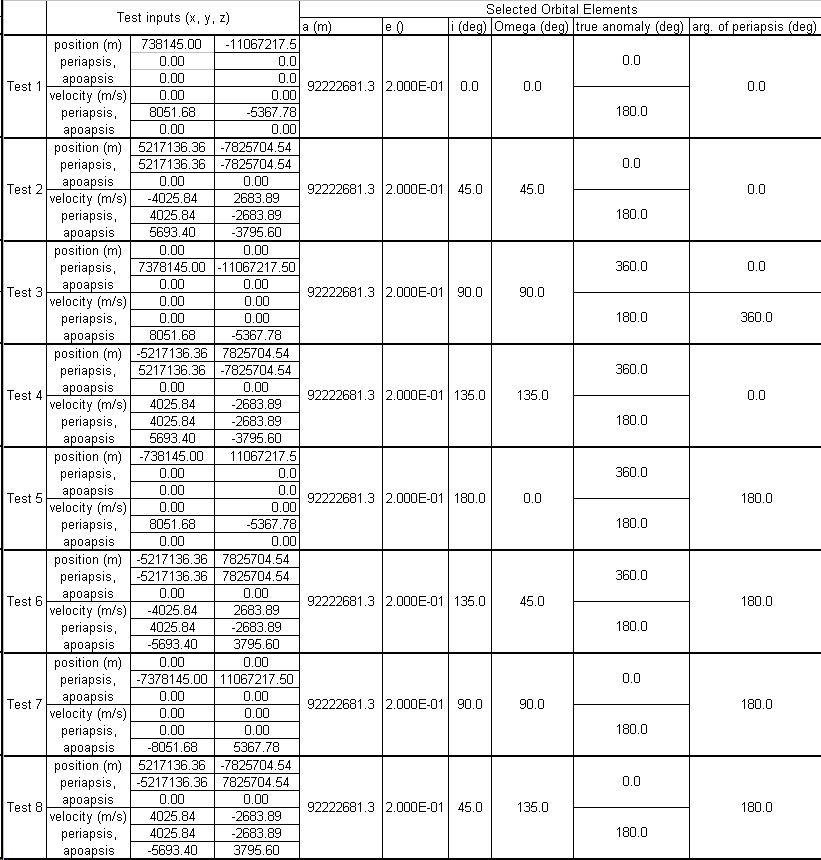
\includegraphics[height=170mm]{JPGfiles/ecc_in_all.jpg}
\caption{Table of Testing Results for Elliptical Orbits}
\label{cir_ecc_all}
\end{center}
\end{figure}

Run directories:

13-20

\end{description}

\test{Conversion to Cartesian Position and Velocity}\label{test:pv_conv}
\begin{description}
\item[Purpose:] \ \newline
The purpose of this test is to examine the performance of the orbital element
to Cartesian position and velocity conversion methods.
\item[Requirements:] \ \newline
By passing this test, the \OrbitalElement\ partially satisfies
requirement~\ref{reqt:elem_convert} and partially satisfies
requirement~\ref{reqt:cart_convert}.
\item[Procedure:]\ \newline
This test is designed to test the conversion from Keplerian orbital elements
to Cartesian position and velocity vectors.  The test itself simply uses the
output from all of the tests described previously and reconverts those orbital
elements to the Cartesian velocity vectors.  If the computation is performed
correctly, the output position and velocity vectors should be exactly the
same as the position and velocity vectors input for all of the previous tests.
\item[Results:]\ \newline
Figure \ref{ele_to_car1} shows a table of the first 8 tests from above
(circular equatorial, and circular polar orbits).  Figure \ref{ele_to_car2}
shows a table of the second 8 tests (circular, 45 degree inclination and RAAN,
and partial elliptical orbits).  And lastly, Figure \ref{ele_to_car3} shows
a table of the final four tests from the elliptical test cases.

\begin{figure}[h]
\begin{center}
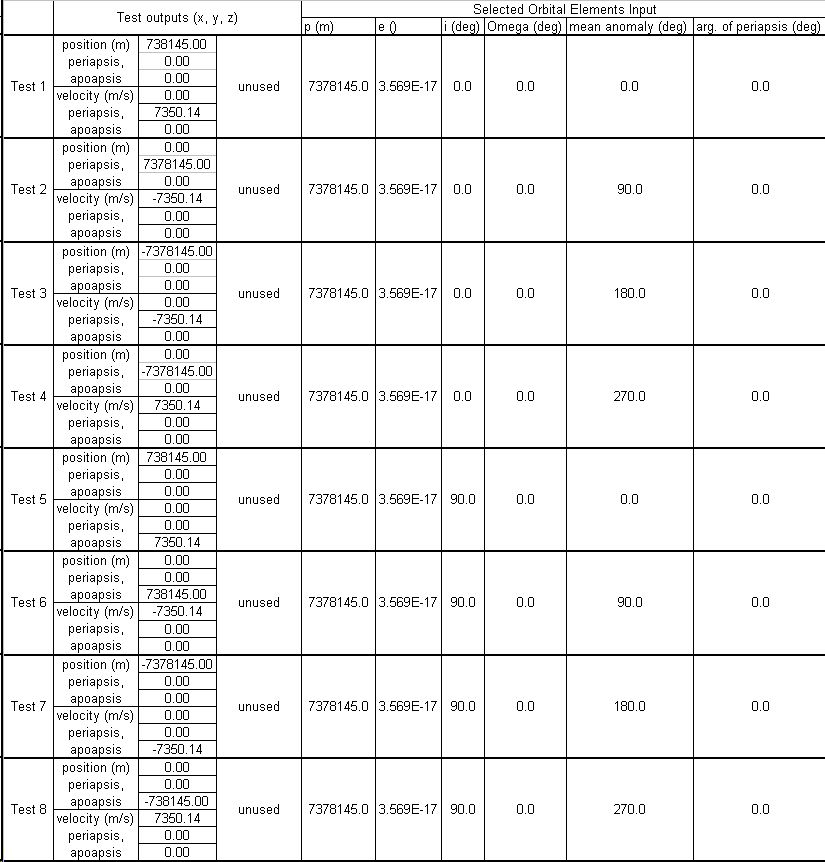
\includegraphics[height=170mm]{JPGfiles/orb_deconvert.jpg}
\caption{First Table of Element to Cartesian Testing Results}
\label{ele_to_car1}
\end{center}
\end{figure}

\begin{figure}[h]
\begin{center}
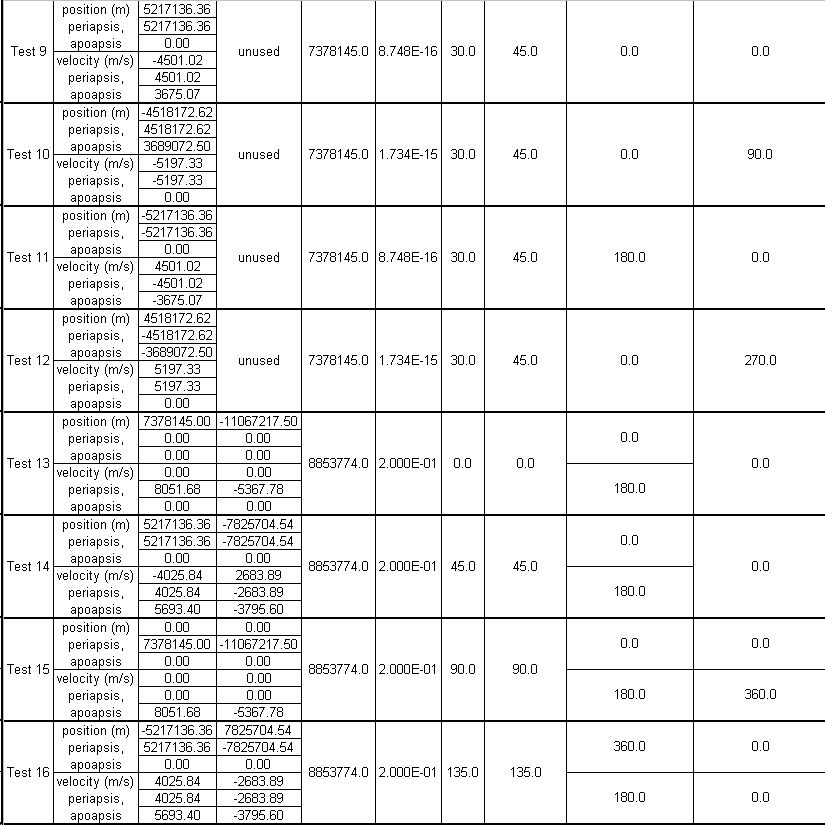
\includegraphics[height=170mm]{JPGfiles/orb_deconvert2.jpg}
\caption{Second Table of Element to Cartesian Testing Results}
\label{ele_to_car2}
\end{center}
\end{figure}

\begin{figure}[h]
\begin{center}
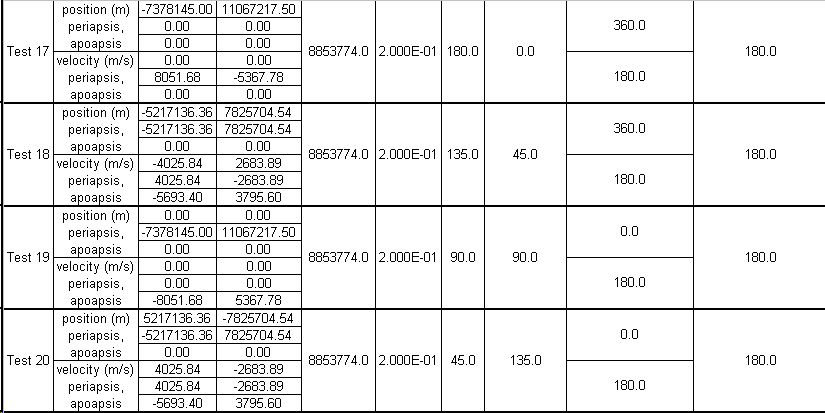
\includegraphics[height=85mm]{JPGfiles/orb_deconvert3.jpg}
\caption{Third Table of Element to Cartesian Testing Results}
\label{ele_to_car3}
\end{center}
\end{figure}

During the course of this testing, several errors in the source code were
discovered.  The errors resulted from numerical instability of the acos C function.
In order to remove this problem, all of the code was modified to use the atan2
function instead of acos to improve the numerical stability of the solution.
Because of this change, the overall performance of the system for these tests
is excellent.  The answers were all consistent to 15 digits of precision which
is the best performance that can be obtained with conventional double precision arithmetic.

Run directories:

21-40
\end{description}

\test{Circular Continuous Orbit}\label{test:circ_cont_orb}
\begin{description}
\item[Purpose:] \ \newline
The purpose of this test is to examine the performance of the orbital element
class with a circular orbit that is not just a single point test.
\item[Requirements:] \ \newline
By passing this test, the \OrbitalElement\ partially satisfies
requirement~\ref{reqt:elem_convert} and partially satisfies
requirement~\ref{reqt:cart_convert}.
\item[Procedure:]\ \newline
This test is designed to examine the \OrbitalElement' performance when
dealing with several continuous data points.  It is run to ensure that there
are no disconnects in the system when dealing with circular orbits and that
there are no clear numerical instability issues.

In order to run this test, a nominal orbit was generated using a MATLAB
propagator (ode45) and simplified system dynamics (two-body problem).  The
trajectory was initialized in a circular orbit and then propagated for a period
of time.  The output position and velocity were then compared with the input
position and velocity.

\item[Results:]\ \newline

Figure \ref{circ_traj_pos_err} shows a plot of the position errors from the
conversion process.

\begin{figure}[h]
\begin{center}
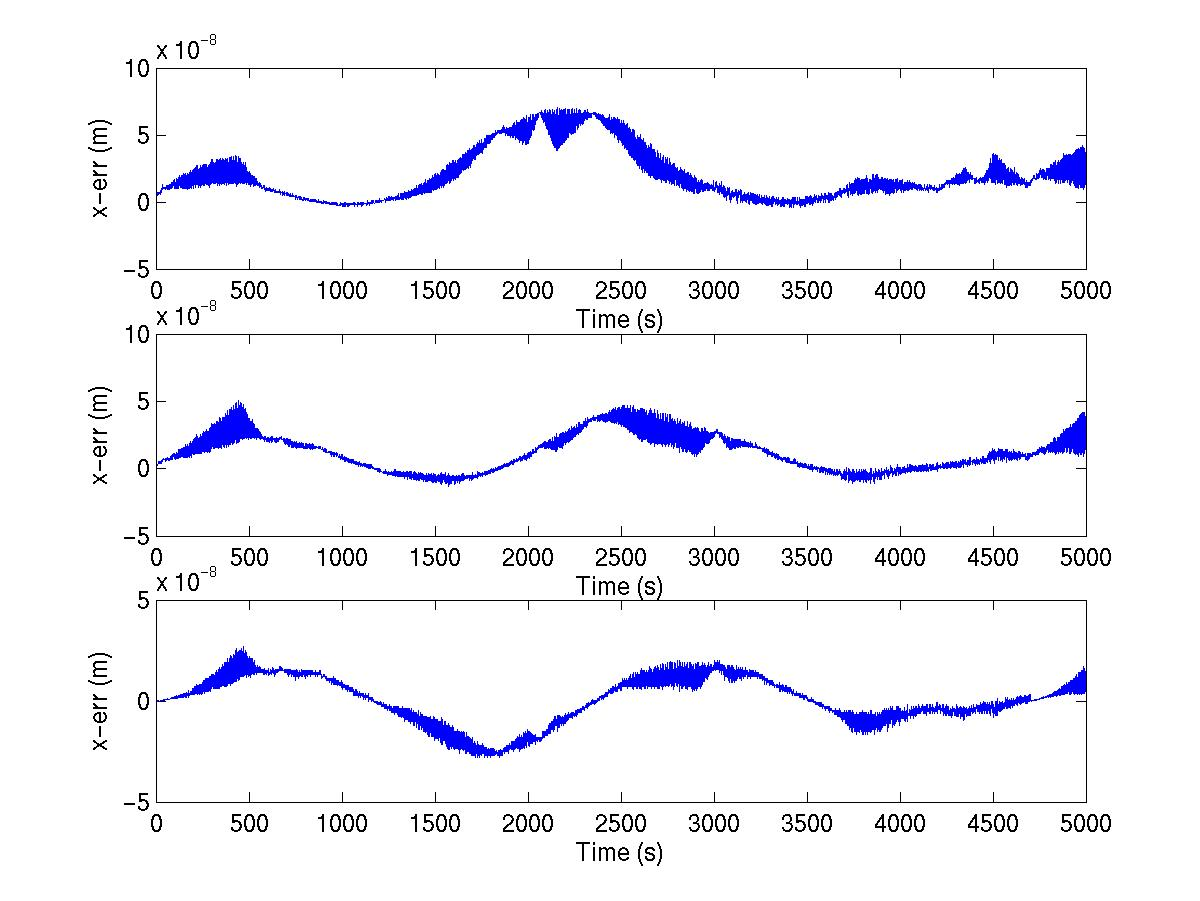
\includegraphics[height=80mm]{JPGfiles/circular_pos_err.jpg}
\caption{Plot of position error for circular orbit}
\label{circ_traj_pos_err}
\end{center}
\end{figure}

As this plot shows, the results all agree to the precision of the computer.
Figure \ref{circ_traj_vel_err} shows a similar plot for the velocity errors
away from nominal.

\begin{figure}[h]
\begin{center}
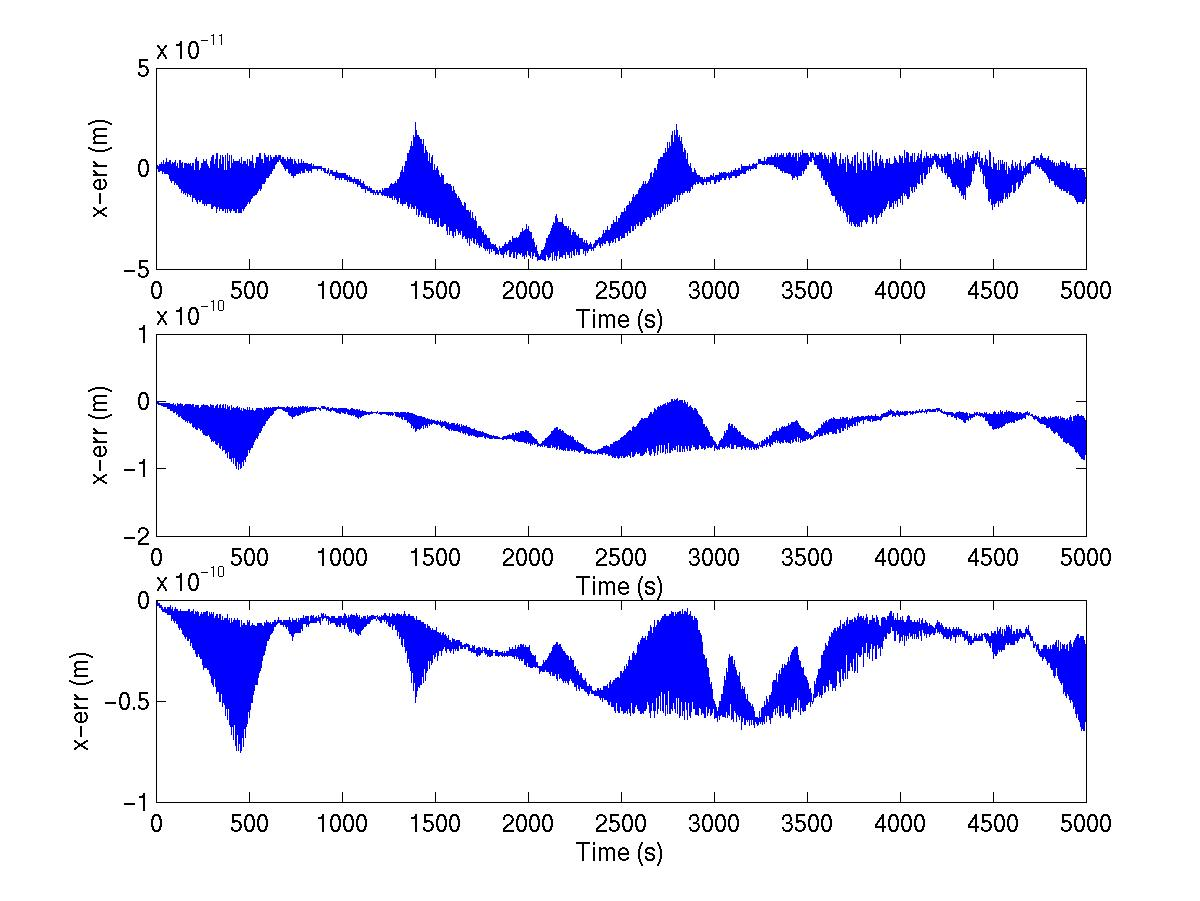
\includegraphics[height=80mm]{JPGfiles/circular_vel_err.jpg}
\caption{Plot of velocity error for circular orbit}
\label{circ_traj_vel_err}
\end{center}
\end{figure}

The velocity performance of the simulation is also quite good.  Figure
\ref{circ_traj_inc_err} shows a plot of the inclination error away from nominal
for this trajectory.

\begin{figure}[h]
\begin{center}
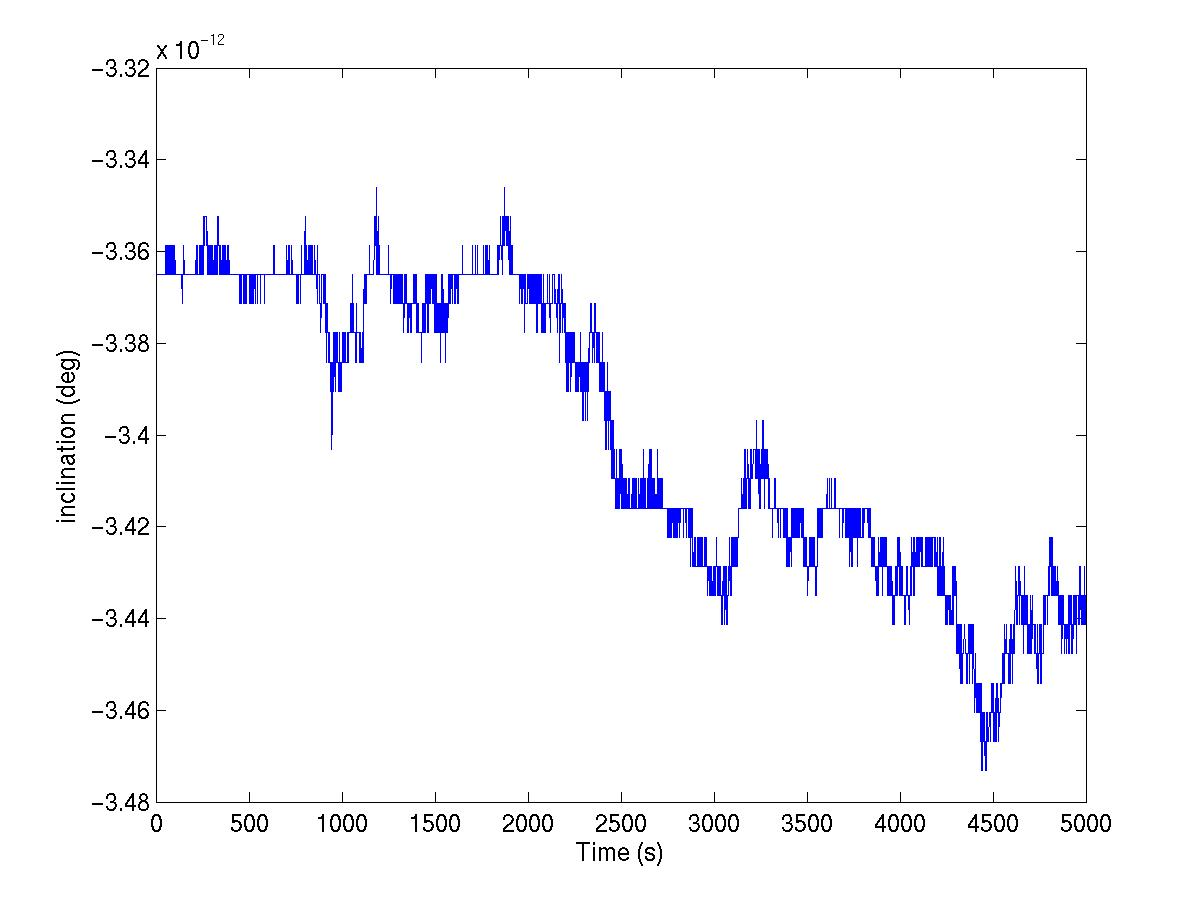
\includegraphics[height=80mm]{JPGfiles/circular_inc_err.jpg}
\caption{Plot of inclination error for circular orbit}
\label{circ_traj_inc_err}
\end{center}
\end{figure}

As these tests show, the \OrbitalElement\ performed nominally for the
tests on the circular orbit problem.

Run directories:

41
\end{description}

\test{Non-Circular Continuous Orbit}\label{test:ecc_cont_orb}
\begin{description}
\item[Purpose:] \ \newline
The purpose of this test is to examine the performance of the orbital element
class with non-circular orbits of varying eccentricity.
\item[Requirements:] \ \newline
By passing this test, the \OrbitalElement\ partially satisfies
requirement~\ref{reqt:elem_convert} and partially satisfies
requirement~\ref{reqt:cart_convert}.
\item[Procedure:]\ \newline
This test is designed to examine the \OrbitalElement' performance when
dealing with several continuous data points.  It is run to ensure that there
are no disconnects in the system when dealing with circular orbits and that
there are no clear numerical instability issues.

In order to run this test, a nominal orbit was generated using a MATLAB
propagator (ode45) and simplified system dynamics (two-body problem).  There
are 8 different eccentricities of the orbit to test all of the possibilities
and borderline cases.

\item[Results:]\ \newline

Figure \ref{ell_cont_pos} shows a plot of the position errors for a continuous
elliptical orbit.

\begin{figure}[h]
\begin{center}
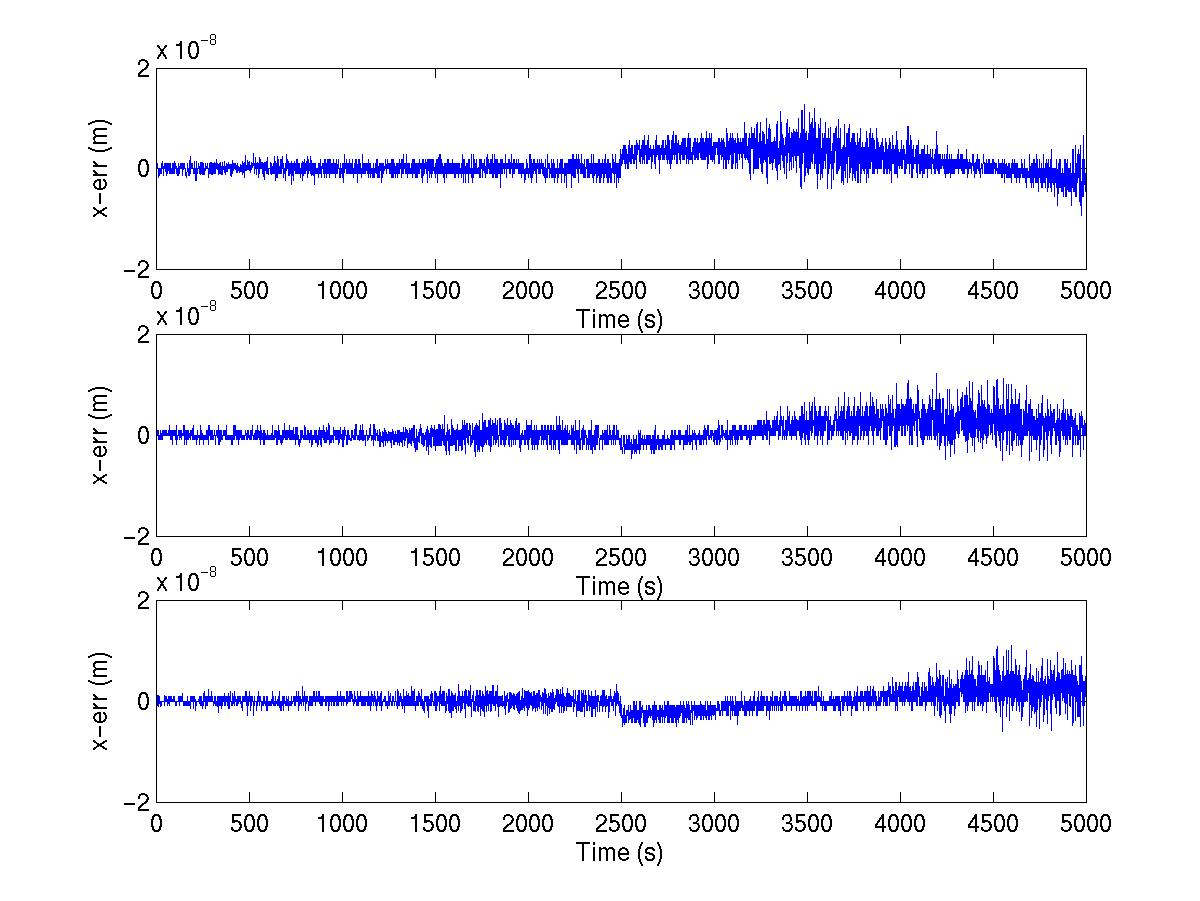
\includegraphics[height=80mm]{JPGfiles/pos_err_ell.jpg}
\caption{Plot of position error for elliptical orbit}
\label{ell_cont_pos}
\end{center}
\end{figure}

Figure \ref{par_low_pos} shows a plot of the position errors in the conversion
for a nearly parabolic trajectory that crosses the border between parabolic
and eccentric trajectories due to propagation errors.

\begin{figure}[h]
\begin{center}
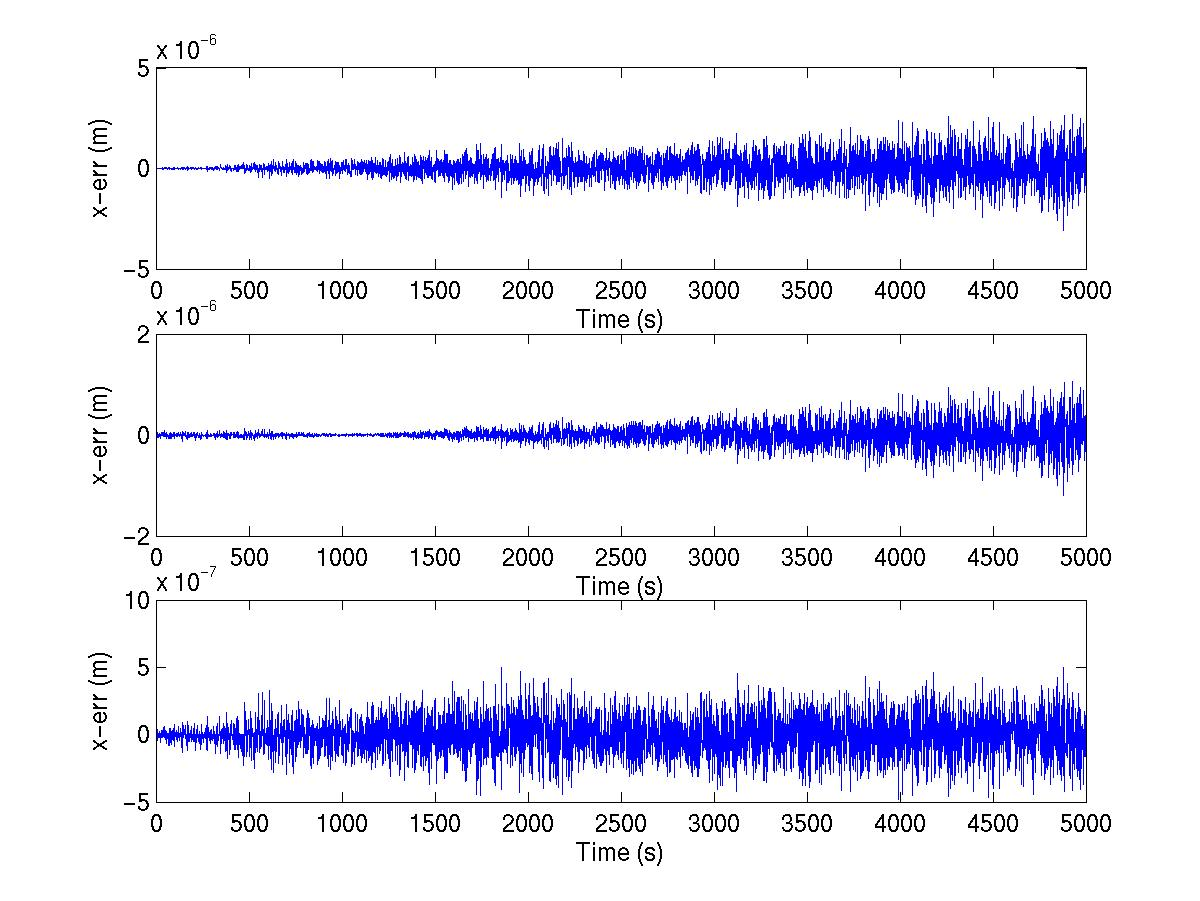
\includegraphics[height=80mm]{JPGfiles/pos_err_par_p99.jpg}
\caption{Plot of position error for low parabolic eccentricity}
\label{par_low_pos}
\end{center}
\end{figure}

Figure \ref{par_mid_pos} shows a plot of the position errors for a parabolic
trajectory that remains in the parabolic region for the entire trajectory.

\begin{figure}[h]
\begin{center}
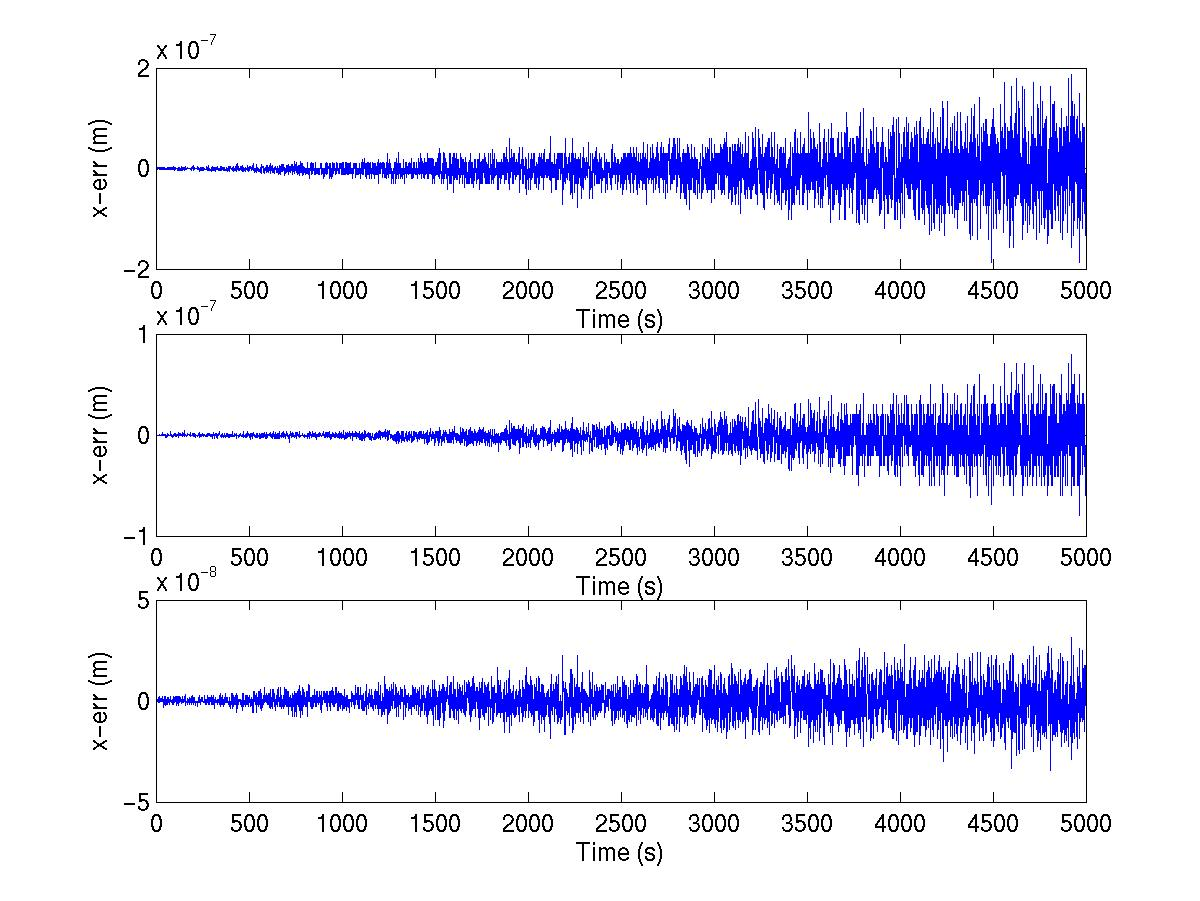
\includegraphics[height=79mm]{JPGfiles/pos_err_par_1.jpg}
\caption{Plot of position error for mid parabolic eccentricity}
\label{par_mid_pos}
\end{center}
\end{figure}

Figure \ref{par_high_pos} shows a plot of the position errors for a parabolic
trajectory that crosses the line between parabolic and hyperbolic trajectories
due to numerical propagation errors.

\begin{figure}[h]
\begin{center}
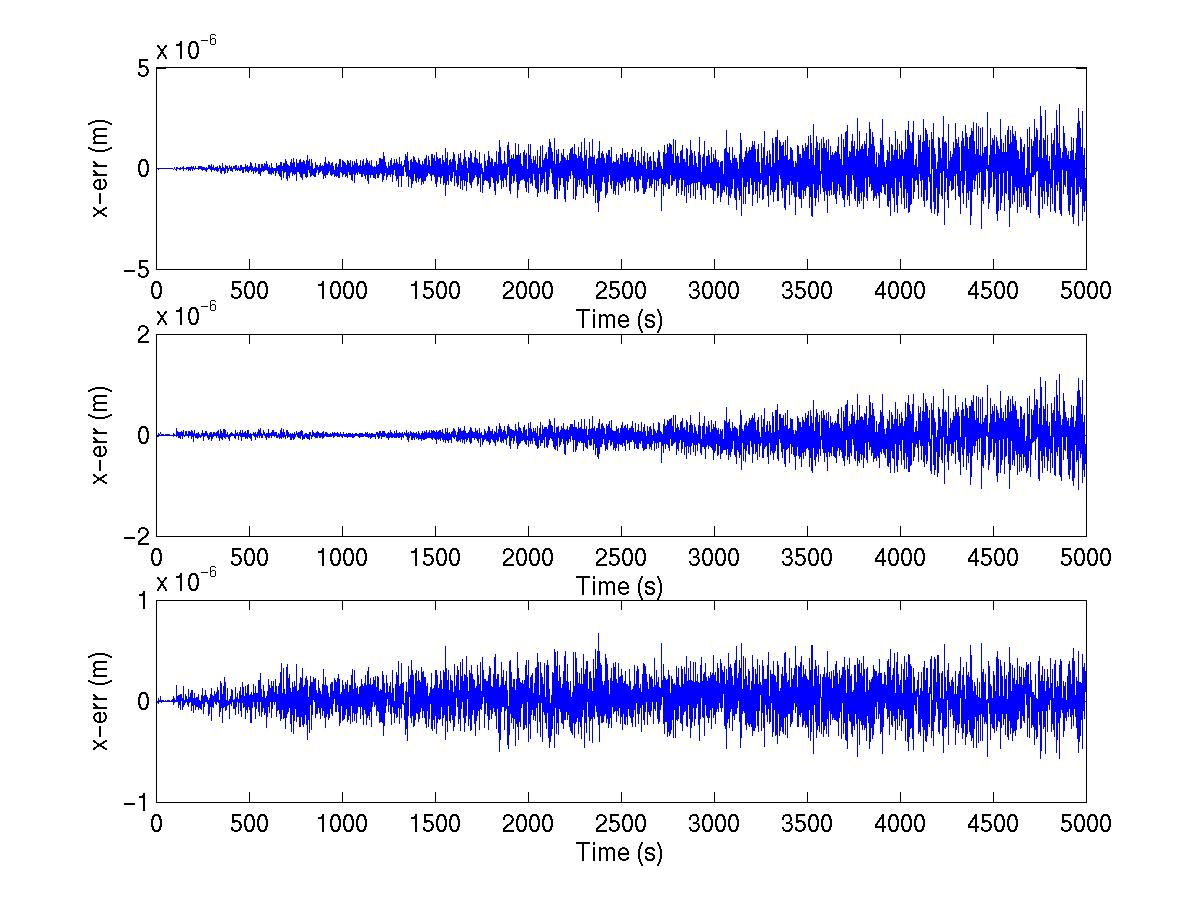
\includegraphics[height=80mm]{JPGfiles/pos_err_par_1p01.jpg}
\caption{Plot of position error for high parabolic eccentricity}
\label{par_high_pos}
\end{center}
\end{figure}

Figure \ref{hyp_low_HM} shows the position errors from a purely hyperbolic
trajectory of eccentricity 1.25.

\begin{figure}[h]
\begin{center}
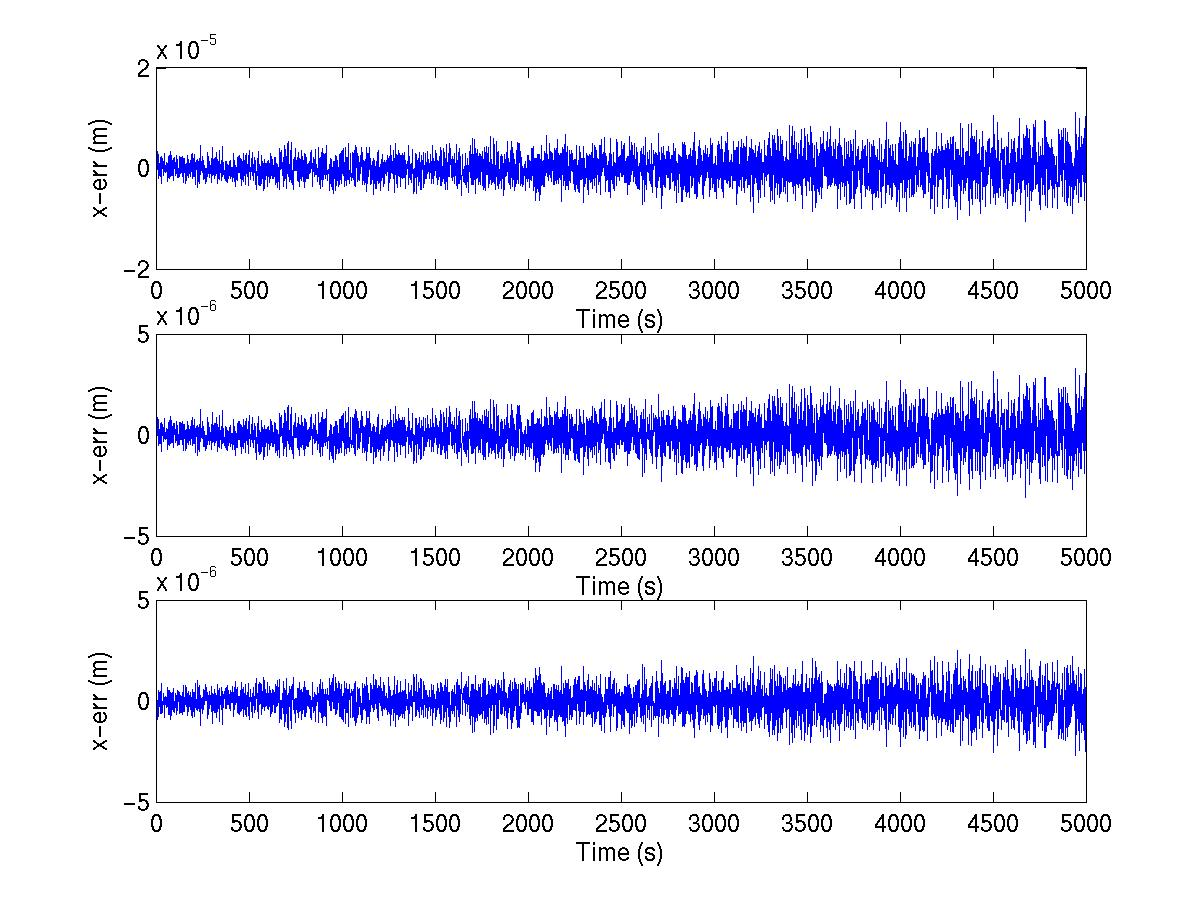
\includegraphics[height=80mm]{JPGfiles/pos_err_hyp_1p25_HM.jpg}
\caption{Plot of position error for hyperbolic eccentricity 1.25}
\label{hyp_low_HM}
\end{center}
\end{figure}

Figure \ref{hyp_mid_HM} shows the position errors from a purely hyperbolic
trajectory of eccentricity 2.5.

\begin{figure}[h]
\begin{center}
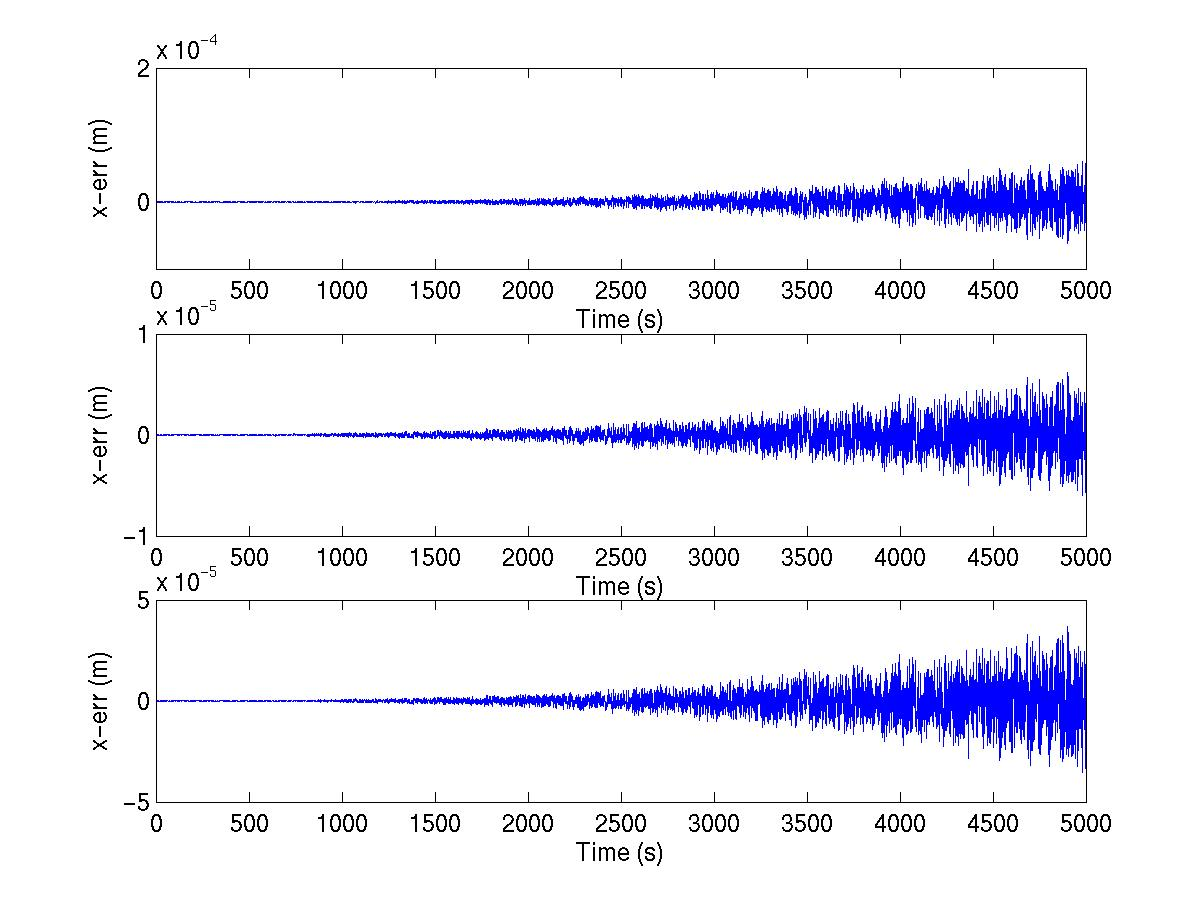
\includegraphics[height=80mm]{JPGfiles/pos_err_hyp_2p5_HM.jpg}
\caption{Plot of position error for hyperbolic eccentricity 2.5}
\label{hyp_mid_HM}
\end{center}
\end{figure}

Figure \ref{hyp_high_HM} shows the position errors from a purely hyperbolic
trajectory of eccentricity 3.9.

\begin{figure}[h]
\begin{center}
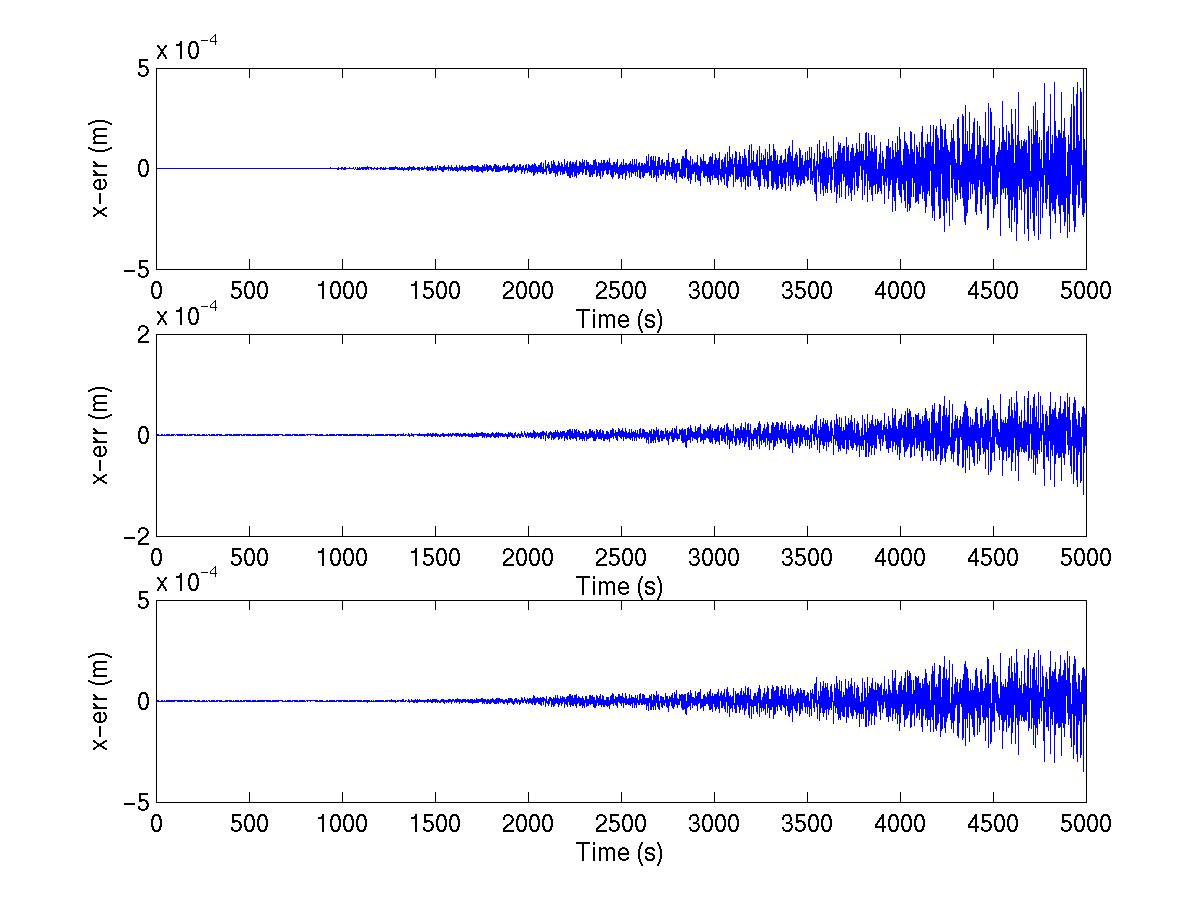
\includegraphics[height=80mm]{JPGfiles/pos_err_hyp_3p9_HM.jpg}
\caption{Plot of position error for hyperbolic eccentricity 3.9}
\label{hyp_high_HM}
\end{center}
\end{figure}

As these plots all show, the \OrbitalElement\ demonstrates good
performance across the board.  In the parabolic region, the digits of
precision are slightly degraded because of numerical instability of the
eccentric orbit calculations in this region.

As part of this testing, the tolerance values from the \OrbitalElement\ had to be
slightly modified.  The tolerance variable that determines when to switch
between eccentric, parabolic, and hyperbolic trajectories was initially
set at 1E-15.  However, when on the border between eccentric and parabolic
orbits, the eccentric orbit calculations experienced numerical instability
because of a subtraction of two numbers that were nearly equal.  When this was
noticed, new tolerance variables were added and the values were tweaked until
the numerical errors in the border region reached a minimum.  The final value
for the type-switching tolerance value was set at 1E-2.

Run directories:

42, 44-50

\end{description}

\test{Published Validation Cases}\label{test:val_case}
\begin{description}
\item[Purpose:] \ \newline
The purpose of this set of tests is to compare the performance of the orbital
element class against published data from other sources (NASA, Vallado, etc).
\item[Requirements:] \ \newline
By passing this test, the \OrbitalElement\ partially satisfies
requirement~\ref{reqt:elem_convert} and partially satisfies
requirement~\ref{reqt:cart_convert}.
\item[Procedure:]\ \newline
This test is designed to compare the \OrbitalElement' performance to
published data from various sources.  There are six tests run.  The first
three are courtesy of NASA's human spaceflight website, the next two are from
Vallado, and the last one is from~\cite{BMW}.

\item[Results:]\ \newline
Figure \ref{val_cases} shows a table of the results from this test.
\begin{figure}[h]
\begin{center}
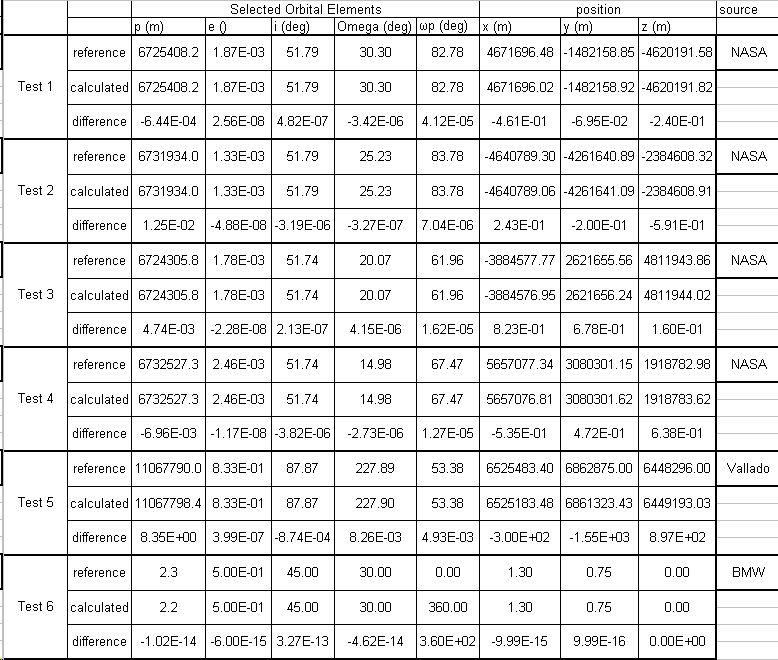
\includegraphics[height=170mm,width=170mm]{JPGfiles/val_case.jpg}
\caption{Validation cases for \OrbitalElement}
\label{val_cases}
\end{center}
\end{figure}

The results from this test are all nominal although it is not apparent at
first.  Particularly, with the Vallado test, where there are only 4 digits
of precision, it does not appear that the methods are particularly accurate
with regards to truth.  However, the Vallado data is only given to four
significant digits so the results shown here are actually nominal.

\end{description}

\test{Code Coverage Test}\label{test:code_coverage}
\begin{description}
\item[Purpose:] \ \newline
The purpose of this test is to ensure that the source code is adequately
covered by the tests run.
\item[Requirements:] \ \newline
By passing this test, the \OrbitalElement\ partially satisfies
requirement~\ref{reqt:elem_convert} and partially satisfies
requirement~\ref{reqt:cart_convert}.
\item[Procedure:]\ \newline
In this test, several different conditions were used to increase the code
coverage of the entire test.  This included things like negative anomalies and
various other tests that should have no effect on the overall simulation.
since the tabulated results do not really add value because they were only
run to increase source coverage, the table has been omitted although it was
examined as part of the testing.

The code coverage obtained through the testing was quite excellent.
checking the results with  the Gnu gcov code coverage tool,
the statement coverage
level was 87\%.  The only reason that coverage was not 100\% is that some of
the code failure cases where the system quits the simulation were not tested.

After this test, all requirements are entirely satisfied.


\end{description}

\section{Requirements Traceability}\label{sec:traceability}

\begin{tabular}{||l|l|l|} \hline
{\bf Requirement} & {\bf Inspection or test} \\ \hline \hline
\ref{reqt:cart_convert} - Cartesian to Element Conversion &
  Insp. \ref{inspect:data_conversion} - file inspection, \\
 & All Tests \\ \hline
\ref{reqt:elem_convert} - Element to Cartesian Conversion &
   Insp. \ref{inspect:data_conversion} - file inspection, \\
 & All Tests \\
\hline
\end{tabular}

\section{Metrics}\label{sec:metrics}
\subsection{Code Metrics}
Table~\ref{tab:coarse_metrics} presents coarse metrics on the source
files that comprise the model.

\input{coarse_metrics}
\newpage
Table~\ref{tab:metrix_metrics} presents the extended cyclomatic complexity
(ECC) of the methods defined in the model.

\input{metrix_metrics}
